\documentclass{article}
\usepackage{graphicx}
\usepackage{amssymb}
\usepackage{amsmath}
\usepackage{tikz}
\usepackage{url}
\usepackage{color}
\usepackage{savetrees}
\usepackage{listings}
\usetikzlibrary{shapes}


\linespread{1.5}
\setlength{\parindent}{0pt}
\setlength{\parskip}{1.9ex plus 0.5ex minus 0.2ex}

\title{CSE638 \\ Advanced Graduate Algorithms (and Data Structures) -- Homework-3}

\author{Dhruv Matani (108267786) \& Gaurav Menghani (108266803)}

\begin{document}
\maketitle

\clearpage

\tableofcontents

\clearpage

\section{Weight Balanced Search Tree}

\subsection{Search cost: $O(\log{n})$}

Since the tree is \textit{weight balanced}, the number of nodes in the
left subtree is a constant fraction away from the number of nodes in
the right subtree. This means that the tree is also height balanced
(i.e. the height of the left and right subtrees are within constant
fractions of each other).

Hence, any root to leaf path in such a tree will not touch more than
$O(\log{n})$ nodes.

\subsection{Worst case update cost: $O(\log{n})$}

To update such a structure, we use \textit{tree rotations}. The
rotations are similar to the \textit{AVL Tree Rotations} we perform to
balance an AVL Tree.

On an insert, we check if the balance conditions are met. If they are,
we don't perform any rotations, and move up to the parent root and
check the balance at the parent node.

Once we find a node that is out of balance, we need to perform either
a single left (or right) rotation or 2 rotations in succession. The 2
cases we need to handle (which are symmetric) are:

\begin{enumerate}
\item If the right child is heavier than the left child and the left
  child of the right child of the imbalanced node is heavier than its
  right sibling, we perform a right rotation around the right child of
  the current node followed by a left rotation around the current
  node.

\item If the right child is heavier than the left child and the left
  child of the right child of the imbalanced node is NOT heavier than its
  right sibling, we perform a single left rotation around the current
  node.

\end{enumerate}

\subsection{Amortized update cost: $O(\log{n})$ (rebalance whole subtree below a node)}

To rebalance a node by re-creating the subtree under it, we perform an
$O(n)$ operation to find the median of the subtree to be re-written
and make the subtree as balanced as possible. The cost to update a
subtree is therefore:

Cost to update =
$\dfrac{\#\ of\ nodes\ to\ rewrite}{\#\ of\ nodes\ that\ caused\ subtree\ to\ go\ out\ of\ balance}$

$=\dfrac{\Theta(n)}{\Omega(n)} = O(1)$

However, since updating a node causes all the subtrees along the
root-to-leaf path of which it is a part to go out of balance, we
charge this node $\Theta(\log{n}) * O(1)$ per update
$=\Theta(\log{n})$.

\clearpage

\section{B-Tree}

\subsection{Search cost: $O(\log{n})$}

The branching factor for such a tree would be $\Theta(c)$, in which
case, the height of the tree is given by the recurrence:

$H(n) = H(n/c) + 1$

$\Rightarrow H(n) = \Theta\left(\dfrac{\log{n}}{\log{c}}\right)$

$\Rightarrow H(n) = \Theta(\log_c{n})$

$\Rightarrow H(n) = \Theta(\log{n})$

Hence, the search cost in such a tree is $O(\log{n})$.

\subsection{Worst case update cost: $O(\log{n})$}

To update such a tree, adopt different strategies for insertion and
deletion. The specific algorithms for worst-case $O(\log{n})$
insertion and deletion can be found here:
\url{https://en.wikipedia.org/wiki/B-tree}

\subsection{Amortized update cost: $O(\log{n})$ (rebalance whole subtree below a node)}

To rebalance a node by re-creating the subtree under it, we perform an
$O(n)$ operation to walk the tree in sorted order of nodes and
re-create the complete tree using a strategy known as
\textit{bulk-loading}. The cost to update a subtree is therefore:

Cost to update =
$\dfrac{\#\ of\ nodes\ to\ rewrite}{\#\ of\ nodes\ updated\ that\ caused\ subtree\ to\ go\ out\ of\ balance}$

$=\dfrac{\Theta(n)}{\Omega(n)} = O(1)$

However, since updating a node causes all the subtrees along the
root-to-leaf path of which it is a part to go out of balance, we
charge this node $\Theta(\log{n}) * O(1)$ per update
$=\Theta(\log{n})$.

\clearpage

\section{Weight Balanced Trees for Order Queries: aka Order
  Maintenance}

We maintain a linked list of elements as a conceptual tree, with each
node in the linked list containing a tag such that if $X \prec Y
\leftrightarrow tag(X) < tag(Y)$.

If we are going to add $n$ elements to this structure, then our tag
space should be $n^c$ for some constant $(c \ge 2)$. This ensures that
our tag space is at least a $2^{nd}$-degree polynomial in $n$.

\textbf{Insertion:} Our structure is conceptually a
\textit{weight-balanced tree}. If we want to insert a new node in the
linked list, we do so at the leaf level. Once we have identified the
node after which we want to insert the new new we check if the tag
just greater than the tag of the existing node is taken. If it is not
taken, we assign that tag value to the newly inserted node and insert
it into the structure. If on the other hand, the tag is taken, we
perform some number of rebalances so that we have a free tag that we
can assign to the newly inserted node.

The algorithm for performing rebalances is as follows:

\begin{enumerate}

\item We define something known as \textit{density thresholds}. Each
  interval of size $2^h$ is capable of holding $T^h$ elements, for $(1
  < T < 2)$.

\item \textit{Intervals} in the tree are defined as runs of sizes that
  are powers of 2, such as 1, 2, 4, 8, 16, \ldots{}

\item Find the smallest interval that is within density thresholds and
  re-write it. i.e. Space out the tags as evenly as possible within
  this interval.

\item If the complete sturecture is not within density thresholds,
  allocate a structure such that the tag space now has space for
  ${(2n)}^c$ elements, and re-write the complete structure.

\end{enumerate}

Every element insertion inches $\Theta(\log{n})$ trees away from
balance.

$\therefore$ Cost to update =
$\dfrac{\#\ of\ nodes\ to\ rewrite}{\#\ of\ nodes\ updated\ that\ caused\ subtree\ to\ go\ out\ of\ balance}$

If $T_i$ is the number of nodes under an unbalanced subtree node at
level $i$, then $T_{i+1}$ is the number of nodes at its parent
subtree, which is guaranteed to be within balance. Therefore, the
number of nodes that caused the imaginary subtree at level $i$ to go
out of balance are:

$= T_i - \dfrac{T_{i+1}}{2} = T_i - \dfrac{\alpha T_i}{2} =
T_i\left(1-\dfrac{\alpha}{2}\right)$

$\because T_{i+1} = \alpha T_i$

$\therefore$ Cost to update $= \dfrac{T_i}{T_i(1-(\alpha/2))} = O(1)$

However, since updating a node causes all the subtrees along the
root-to-leaf path of which it is a part to go out of balance, we
charge this node $\Theta(\log{n}) * O(1)$ per update
$=\Theta(\log{n})$.

\textbf{Querying:} Given 2 pointers to elements, to query their
relative order, we just check the relative ordering of their
\textit{tag} values. This is a constant time $O(1)$ operation.

\textbf{$O(1)$ Update:} To get $O(1)$ update, we use the technique of
\textit{indirection}. We cut our imaginary tree so that for a
structure containing $n$ elements, the top tree contains
$\Theta(\frac{n}{\log{n}})$ leaf nodes and the bottom tree contains
$\Theta(\log{n})$ nodes in total.

This means that we update the top tree every $\Theta(\log{n})$
inserts. This gives us an amortized update cost of
$\dfrac{\Theta(\log{n})}{\Theta(\log{n})} = O(1)$.

Since the smaller trees each contain only $\Theta(\log{n})$ nodes, we
can create a tag space of size $n$ (which is exponential in
$\Theta(\log{n})$), so that every insert takes worst-case $O(1)$ time.

Each element now has 2 tags, a \textit{big-tag} and a
\textit{little-tag}. To check if an element precedes another in the
list, we need to check both tags. $X \prec Y \leftrightarrow
(bigtag(X) < bigtag(Y) \vee (bigtag(X) = bigtag(Y) \wedge littletag(X)
< littletag(Y)))$.

\clearpage

\section{Even more \textit{Packed} Memory Array}

Let $N$ be the physical space allocated (capacity) for the PMA.

$\therefore$ the \# of gaps in this PMA are $O(\frac{N}{\log{N}})$.

$\therefore$ the maximum \# of elements that can be stored in such a
PMA are $O(N - \frac{N}{\log{N}}) = O(\frac{N\log{N} - N}{\log{N}})$.

Let's suppose that we can store between $\frac{N\log{N} - N}{2\log{N}}$ \&
$\frac{N\log{N} - N}{\log{N}}$ elements in the PMA.

Hence, the upper density threshold $\tau_h = \dfrac{max\ \#\ of\ elements\ in\ the\ PMA}{capacity\ of\ the\ PMA}$

$= \dfrac{N\log{N} - N}{N\log{N}}$

$= 1 - \dfrac{1}{\log{N}}$

We know that $\tau_0 = 1$.

$\therefore$ the difference between the lower and upper density thresholds = $(\tau_0 - \tau_h) = \dfrac{1}{\log{N}}$

The number of levels in the imaginary tree are $\log{N}$.

Hence, the difference between each level is $\dfrac{1}{\log^2{N}}$.

The cost to rebalance a level is $= \dfrac{\Theta(size\ of\ a\ subtree\ rooted\ at\ that\ node)}{\#\ of\ updates\ that\ cause\ the\ subtree\ to\ go\ out\ of\ balance}$

$= \dfrac{\Theta(subtree\ size)}{size\ of\ subtree\ \times\ difference\ in\ threshold\ between\ 2\ consecutive\ levels}$

$= O(\log^2{N})$

However, since there are $\log{N}$ levels, we need to charge each update $\log{N}$.

$\therefore$ the amortized cost per update is $= O(\log^3{N})$.

\clearpage

\section{Efficient Rebalancing}

\subsection{Moving every element at most twice}

An algorithm that moves every element at most twice will first
compress all the elements to one side (say to the left) and then
expand the elements out from the other side. This is always possible
since we are always compressing or expanding out elements into blank
cells.

\clearpage

\section{PMA with arbitrary rebalance windows}

Instead of rebalancing a PMA at fixed interval windows, we can choose
any interval window to rebalance as long as the size of the intervals
grows exponentially. We adopt a simple approach wherein we start the
interval at the element just before the element being inserted. Hence,
our rebalance window might \textit{wrap around} to the beginning of
the array.

The analysis is simple if we charge updates to \textit{levels} instead
of subtrees rooted at certain levels. Hence, in the fixed-interval
PMA, if we re-balance a subtree rooted at a certain level $l$, we
charge the updated element $\log{N}$ since it causes $\log{N}$
subtrees to inch away from being within threshold. In this version of
the PMA, if we re-balance a subtree rooted at a certain level $l$, we
charge the \textit{level l} instead of charging the subtree rooted at
that level.

It is easy to see that we will charge the root node in the original
PMA the same number of times as we charge imaginary root nodes in the
modified PMA. The aggregate sum of rebalances at any level in the
original and the modified PMA remain the same. Hence, the cost to
update an element remain the same even in the modified PMA.

\clearpage

% External Memory Problems

\section {Number of Memory Transfers to Search and Update a B-Tree}
In the standard B-Tree, all internal nodes (i.e., except the root and
the leaf nodes) have a branching factor (equal to the number of
children it has) between $\frac{B}{2}$ and $B$. All internal nodes
have the number of elements which is one less than the number of
children, and the elements are stored in a sorted order. $B$ is chosen
to co-incide with the size of a block.

The elements in a node necessarily partition the elements stored in
the sub-trees of the node. Since there are $\Theta(B)$ pivots, the
range of the search becomes smaller by a factor of $\Theta(B)$ at
every level. Therefore, the number of levels in the search tree would
be $\log_B{N}$, and since the cost of transfering all the elements of
a node into memory is one block transfer, the overall memory transfers
required for searching is $O(\log_B{N})$.

Once we have found the node where the element exists, we will either need to split
or merge the node, where the element exists. This is an $O(1)$ memory transfer operation.

Thus, once the node has been found, the cost for update is $O(1)$.

\clearpage 

\section {Lower Bound on Memory Tranfers for Searching in the DAM Model}
If we have a set of $N$ sorted elements, with each block transfer, the best we can
do is to get $B$ elements, each of which acts as a pivot and together they partition
the current range into $B+1$ sub-ranges of equal sizes. 

After comparing our target element with each of the pivots, we can make a decision
about the sub-range to search in, which would now be smaller by a factor of $B+1$.
Thus, the depth of the recursion tree would be $O(\log_B{N})$, and since each level
requires us to make one memory transfer, the lower bound on the number of memory
transfers for Searching in the DAM model is $\Omega(\log_B{N})$.

\clearpage

\section {The cost to build a B-Tree is $\Theta\left(\left\lceil\dfrac{N}{B}\right\rceil\right)$}
In a B-Tree with $N$ elements, a fraction of $\frac{B-1}{B}$ resides in the leaves, and
the rest of the $\frac{1}{B}$ elements reside in the upper tree. 

The algorithm to build a B-Tree would be:
\begin{enumerate}
\item If the number of elements in the current array $N \leq B $, stop.
\item Allocate space for $\frac{N}{B}$ elements in a temporary array.
\item Scan through the array, copy the first $B-1$ elements into a new node.
\item Copy the next element into a parent block. 
\item Mark the newly created node as the child of the element inserted in the parent block.
\item If the parent block has $B$ elements, append it into the temporary array.
\item If there are no more elements left to be seen in the current array, set the temporary
array as the new current array, and go to step 1.
\item Else, if there are elements left to be seen in the current array, and go to step 3.
\end{enumerate}

We see that, for each iteration, if the size of the current array is $N$, we incur
$\frac{N}{B}$ memory transfers for scanning through the array and creating new nodes
, and $\frac{N}{B^2}$ for copying elements into the temporary array. The recursion
can be seen as follows:\\

$T(N) = T(\frac{N}{B}) + \Theta(\frac{N}{B})$ \\
$T(B) = 1$\\
\\
Clearly, the solution of the recursion is $T(N) = \Theta\left(\dfrac{N}{B}\right)$, but since we cannot
make a fractional number of memory transfers, we round up the number of memory transfers
to $\left\lceil \dfrac{N}{B} \right\rceil$.

\clearpage

\clearpage

\section {Search and Modify cost in a Weight-Balanced B-Tree}
The search cost in a Weight-Balanced B-Tree remains the same as the usual
B-Tree, since each node still has $\Theta(B)$ elements, and hence the cost still is
$O(\log_B{N})$.

Let us define the weight of a tree rooted at a node $u$, by $w(u)$, which is the
number of nodes in the sub-tree rooted at $u$. Since the B-Tree is weight-balanced,
the number of updates between a rebalance is $\Omega(w(u))$. Thus the 
amortized number of elements touched / update at each level would be: 
$\dfrac{O(w(u))}{\Omega(w(u))}$, which would be $O(1)$ amortized / level. 

Since there are $O(\log_B{N})$ levels, the total amortized number of elements 
touched / update would be $O(\log_B{N})$, and thus the amortized number of memory transfers
would be $O\left(\dfrac{\log_B{N}}{B}\right)$.

Therefore, the total amortized number of memory trasfers for search and modify would
be $O(\log_B{N}) + O\left(\dfrac{\log_B{N}}{B}\right)$
\clearpage

\section {Rebalancing scheme for a Weight-Balanced Tree with Splits and Merges}
TODO: Fill Up

\clearpage

\section{External Sorting}

We have $N$ elements and $B$ is the number of numbers in a
block. Hence, we have $\frac{N}{B}$ blocks.\\ Let $X =
\frac{N}{B}$. Also, let the number of blocks that we can fit in main
memory be $Y = \frac{M}{B}$.
\\
Since we are only interested in the number of blocks being
transferred, we don't worry about the actual computational complexity
of performing the sort (or merge).\\

\subsection{Algorithm Description}

\begin{enumerate}
\item We start off by assuming the input to be $X$ blocks of
  integers. We only deal in number of blocks from now.
\item We start off with $X$ \textit{runs} which contain $1$ block
  each.
\item Read in $Y$ blocks of input and merge them
  \textit{in-place}. We store metadata about each sequence's end so
  that we know when we run out of numbers in a block.
\item Once we run out of numbers in a block, we shall read off one more
  block from the same \textit{run} from which this block
  originated. If no more blocks exist in this run, we do nothing and
  wait for some other block to become empty.
\item As soon as a block becomes empty, we write it out to
  disk. Continuous write like this will result in a sorted sequence of
  blocks that are $Y$ more in ratio than the number of blocks in the
  input. For example, if we have $Y = 4$ and we start off with $32$
  runs of size $1$ block each, then we land up with $8$ runs of size
  $4$ blocks each after the first round, $2$ runs of size $16$ after
  the second round, and so on \ldots{}
\item Once we completely exhaust all blocks in a run, we then start
  processing the next set of $Y$ runs.
\item It is easy to see that we are reducing the number of runs by a
  factor of $Y$ at every stage. Hence, the size of the recursion tree
  will be at most $Y$ in depth.
\end{enumerate}

\subsection{Recurrence Relation}

$T(X) = YT(\frac{X}{Y}) + X$\\
The factor $X$ is added to the recurrence since we need to read off
$X$ blocks of integers at every stage.\\
$\Rightarrow T(X) = O(X^{\log_Y{Y}}\log_Y{X})$\\
Re-substituting, we get:\\
$\Rightarrow T(N/B) = O(\frac{N}{B}\log_{\frac{M}{B}}{\frac{N}{B}})$\\
\\
Each number in the boxes in the figure represents a single
\textit{block} of input, and each box represents a single
\textit{run}. Each \textit{run} may contain multiple
\textit{blocks}. We assume that $Y = 2$ for the figure below.

\begin{center}
  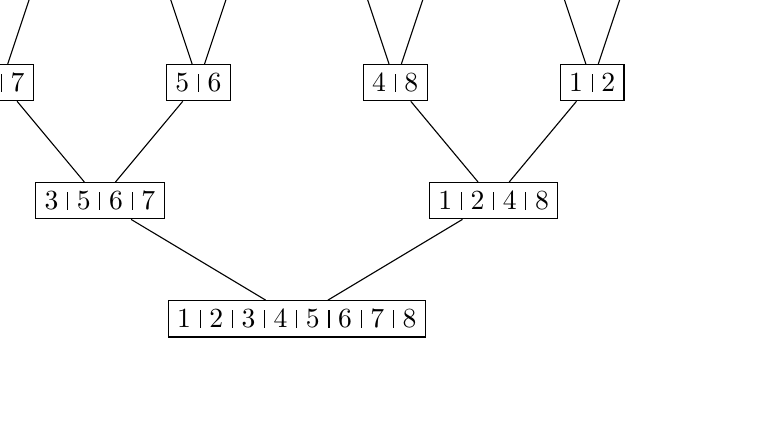
\begin{tikzpicture}
    \tikzstyle{every node}=[rectangle,draw]
    \tikzstyle{level 1}=[sibling distance=50mm]
    \tikzstyle{level 2}=[sibling distance=25mm]
    \tikzstyle{level 3}=[sibling distance=10mm]
    \node[rectangle,draw] {1 \vline \ 2 \vline \  3 \vline \  4 \vline
      \  5 \vline \  6 \vline \ 7 \vline \ 8} [grow'=up]
    child {node {3 \vline \ 5 \vline \  6 \vline \  7}
      child {node {3 \vline\ 7}
        child {node {3}}
        child {node {7}}
      }
      child {node {5 \vline\ 6}
        child {node {6}}
        child {node {5}}
      }
    }
    child {node {1 \vline \ 2 \vline \ 4 \vline \  8}
      child {node {4 \vline\ 8}
        child {node {8}}
        child {node {4}}
      }
      child {node {1 \vline\ 2}
        child {node {2}}
        child {node {1}}
      }
    }
    ;
  \end{tikzpicture}
\end{center}


\clearpage


\section{Matrix Multiplication}

\subsection{Divided into blocks of size $B$}

Suppose we are given an $N \times N$ matrix $A$, and another $N \times
N$ matrix $B$, and we are asked to find the product of the 2, we can
use the divide \& conquer algorithm to do so. We can split both
matrices into 4 parts and consider it to be a matrix multiplication of
two $4 \times 4$ matrices.

\[
Product =
\begin{pmatrix}
  a_{1,1} & a_{1,2} \\
  a_{2,1} & a_{2,2} 
\end{pmatrix}\times
\begin{pmatrix}
  b_{1,1} & b_{1,2} \\
  b_{2,1} & b_{2,2} 
 \end{pmatrix}
\]
\\
The number of multiplications needed for this is $8$.\\
\\
Now, if our matrix is stored such that when we reach a matrix of size
less than or equal to $\sqrt{B} \times \sqrt{B}$, we store that
complete matrix in one chunk rather than split the rows. If we store
the matrix in such a manner than multiplying two matrices with sizes
$\sqrt{B} \times \sqrt{B}$ each can be done using a constant number of
disk operations.\\
\\
This means that the number of matrices of size $\sqrt{B} \times
\sqrt{B}$ in the original matrix are $\frac{N}{\sqrt{B}}$. Hence, we get the
following recurrence for the number of multiplications required:\\
\\
$T(n) = 8T(\frac{n}{2}) + O(n^2)$\\
Substituting $n = \frac{N}{\sqrt{B}}$, we get the number of disk
transfers required:\\
$\Rightarrow T(n) = 8T(\frac{N}{2\sqrt{B}}) + O(\frac{N^2}{B})$\\
$\Rightarrow T(n) = \frac{N^3}{\sqrt{B}^3}$\\
$\Rightarrow T(n) = \frac{N^3}{{B}^{3/2}}$

\subsection{Divided into blocks of size $M$}

If we divide the matrix into blocks of size M (i.e. a matrix of size
$\sqrt{M} \times \sqrt{M}$, then we get $\frac{N}{\sqrt{M}}$ matrices
(or blocks) at the lowest level. Each such matrix can be read off from
the disk in time $O(\frac{M}{B})$.\\
\\
Hence, the recurrence for the number of disk transfers is:\\
$T(n) = \frac{M}{B} \times T'(n)$\\
$T'(n) = 8T(\frac{N}{2\sqrt{M}}) + O(\frac{N^2}{M})$\\
$\Rightarrow T(n) = \frac{M}{B} \times \frac{N^3}{M^{3/2}}$\\
$\Rightarrow T(n) = \frac{N^3}{B\sqrt{M}}$


\clearpage

\section{Matrix Multiplication}

\subsection{Recursion relation for the cost of a multiplication}

$T(n) = 8T(\frac{n}{2}) + O(n^2)$\\

\subsection{Number of memory transfers for divide \& conquer
  multiplication}

To compute the number of memory transfers for divide \& conquer
multiplication, we need to find out the number of memory transfers
required for multiplying 2 matrices of size $\sqrt{M} \times \sqrt{M}$
each (which is $\frac{M}{B}$) and multiply that by the number of
multiplications of matrices of size $\sqrt{M} \times \sqrt{M}$ needed
to multiply two matrices of size $N \times N$. This turns out to be:\\
\\
$T(n) = \frac{M}{B} \times T'(n)$\\
$T'(n) = 8T(\frac{N}{2\sqrt{M}}) + O(\frac{N^2}{M})$\\
$\Rightarrow T(n) = \frac{M}{B} \times \frac{N^3}{M^{3/2}}$\\
$\Rightarrow T(n) = \frac{N^3}{B\sqrt{M}}$


\clearpage

% van Emde Boas problems
\section{Deletions in vEB Tree}
Find the predecessor and successor of the element to be deleted. Let us call them $p$, $s$,
and $e$ respectively. 

Now traverse down the path of the vEB tree with $e$ as the index. If $p$ and $s$ belong to the
same widget, then just recusively delete the element $e$ from the child widget. If $p$ does not
belong to the current widget, but $s$ does, set the min of the current widget to $s$. If $s$ does
not belong to the current widget, but $p$ does, set the max of the current widget to $p$. If 
neither of them exist, then mark the min and max of the current widget as -$\infty$ and +$\infty$
respectively, and recurse. 
(TODO: Verify)

\clearpage

\section{vEB Trees in $O(n)$ space}

The naive version of vEB tree takes $O(u)$ space. However, this is
wasteful since, not all the widgets would be in use at the very same
time. From the Hashing lecture in class, we know that we can hash $n$
elements in $O(n)$ space, while maintaining $O(1)$ query time.

Now, instead of explicitly maintaining all $\sqrt{u}$ sub-widgets, and
the summary widget, we maintain only the summary widget explicitly for
a widget, and allocate sub-widget as required.  To aid us, we create a
dynamic hash-table on the sub-widget index ($X_H$), and when we need
to insert in a sub-widget for the first time, we allocate space for it
dynamically, and insert the sub-widget index ($X_H$) in the table,
with the value being the memory location of the newly allocated
widget.

Now, instead of indexing into the array as we did earlier for a
widget, we now lookup in the hash-table to find the location where we
have stored the widget, and inspect the widget at that location, and
proceed appropriately. The rest of the algorithm remains the
same. However, the running time is now \textit{with high probability}
instead of deterministic worst-case.


\end{document}
